\section{Aufbau des Informationsmanagements nach Krcmar - AD}
\label{section_aufbau_des_informationsmanagements_nach_krcmar}

Prof. Dr. Helmut Krcmar, 1954 in Hanau geboren, schloss sein Studium der Wirtschaftswissenschaften an der Universität des Saarlandes ab und hat derzeit den Lehrstuhl der Wirtschaftsinformatik der Technischen Universität München inne.

Im Rahmen seines beruflichen Werdeganges widmete er sich der Forschung  auf dem Gebiet der Wirtschaftsinformatik, insbesondere dem Informationsmanagement.

Krcmars Ziel ist es, eine fokussierte und strukturierte Darstellung der Grundzüge des Informationsmanagements zu geben, mit dem Fokus auf der Präsentation ausgewählter Themen, Methoden und Konzepten.

Als Autor verschiedener veröffentlichter Werke hat Krcmar die Ansichtsweise des
Informationsmanagements in Deutschland revolutioniert. Aus seiner Hand stammen die
meisten Publikationen zum Thema Informationsmanagement aus informationstheoretischer
Perspektive.\footcite{marsch_krcmar_2015}

Das Informationsmanagement hat als primäre Aufgabe die betriebswirtschaftlich sinnvolle Steuerung von Informationen, die nach Krcmar als Ressource beschrieben werden.

Die Gestaltungsmöglichkeiten der innerbetrieblichen Informationswirtschaft im Spannungsfeld zwischen dem technologisch Realisierbarem, den arbeitsorganisatorischen Anforderungen der Mitarbeiter an Informationssysteme, der organisatorischen Konfiguration selbst und dem wettbewerblichen Umfeld der Organisation geben dem Informationsmanagement Bedeutung.\footcite{fortiss_krcmar_2015}

Der Autor verfolgt das Ziel, eine fokussierte und strukturierte Darstellung der Grundzüge des Informationsmanagements zu geben. Das Informationsmanagement ist laut seiner Definition eine Managementaufgabe.

Drei Kernbereiche sind hier zu berücksichtigen.
\begin{enumerate}
	\item Das Management der Informationswirtschaft
	\item Das Management der Informationssysteme
	\item Das Management der Informations- und Kommunikationstechnik
\end{enumerate}

Das Informationsmanagement in die Organisations-, Führungs- und Kontrollstrukturen zu integrieren unterliegt dem Management der Unternehmensführung.

In seinen Werken definiert Krcmar einleitend die Grundbegriffe des Informationsmanagements.

\paragraph*{Information}\mbox{}\\\\
Das Wort „Information“ ergibt sich auf Grund einer Abbildung \ref{fig_ebenen_begriffshierarchie}, die den Zusammenhang zwischen Zeichen, Daten, Informationen und Wissen auf vier Ebenen darstellt.

\begin{figure}[h!]
	\centering
	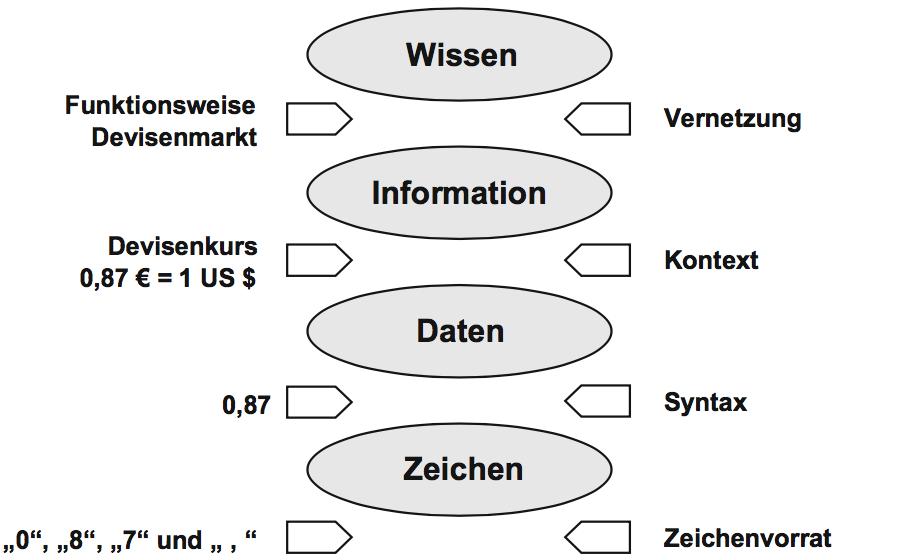
\includegraphics[width=11cm]
	{kapitel/gruppe1_1/bilder/ebenen_der_begriffshierarchie_neu}
	\caption{Die Beziehungen zwischen den Ebenen der Begriffshierarchie nach Krcmar\protect\footnotemark}
	\label{fig_ebenen_begriffshierarchie}
\end{figure}\footnotetext{\cite{krcmar_einfuhrung_2015}}

Wie in Abbildung \ref{fig_ebenen_begriffshierarchie} zu erkennen ist, befindet sich auf der untersten Ebene ein Zeichenvorrat als Basis aller weiteren oben angesiedelten Begriffe. 
Aus diesem Zeichenvorrat entstehen Daten, wenn die Zeichen in einen definierten, strukturierten Zusammenhang gebracht werden.
Werden diese entstandenen Daten mit Kontext angereichert, bekommen sie eine Bedeutung, sodass eine Information entsteht. 
Durch die Vernetzung dieser Information mit anderen Informationen entsteht Wissen auf einer übergeordneten Begriffshierarchie.

Wird Information als Produktionsfaktor im betrieblichen Leistungsprozess angesehen, 
versteht sie sich in diesem Zusammenhang als eine immaterielle, aber nicht kostenlose Ressource.

Des Weiteren bringen Informationen dem Verwender einen Nutzen, wenn sie in Handeln umgesetzt werden. Informationen sind keine keine freien Güter, weshalb sie keinen kostenadäquaten Wert haben können.

Der Wert hängt von der kontextspezifischen und zeitlichen Verwendung ab. Sie sind darüber hinaus auch erweiterbar und verdichtbar. Über die Qualität entscheiden mehrere Einflussfaktoren, wie beispielsweise die Vollständigkeit, die Genauigkeit und die Zuverlässigkeit.

Informationen werden kodiert übertragen, weshalb für ihren Austausch gemeinsame Standards notwendig sind.

\paragraph*{Management}\mbox{}\\\\
Im funktionalen Sinne beschreibt das Management spezielle Aufgaben und Prozesse, die unternehmensintern und zwischen Unternehmen stattfinden.
Diese Aufgaben werden wiederum unterteilt in Personalfunktionen und Fachfunktionen. In den Aufgabenbereich der Personalfunktionen fallen die persönliche Betreuung, sowie die soziale Integration der Mitarbeiter, im Sinne der Arbeitsplatzgestaltung und der Personalförderung.

Aus den Fachfunktionen lässt sich die Unterstützung an der Realisierung der Unternehmensziele ableiten. Planung (Zielvorgabe, Problemanalyse, Alternativensuche), Entscheidung sowie Realisierung und Kontrolle stehen im Mittelpunkt.
Dem Management als Institution gehören alle Personen an, die als Entscheidungsträger ständig personen- und sachbezogene Aufgaben wahrnehmen: Vorstand, Führungskräfte, Stäbe.

\paragraph*{Informationssysteme}\mbox{}\\\\
Bei Informationssystemen (IS) handelt es sich um soziotechnische („Mensch-Maschine-“) Systeme, die menschliche und maschinelle Komponenten (Teilsysteme) umfassen und zur Bereitstellung von Informationen und Kommunikation nach wirtschaftlichen Kriterien eingesetzt werden.

Planung und Bereitstellung der Informationssysteme des Unternehmens zur Erfüllung betrieblicher Aufgaben stellen damit einen Teilbereich der Informationsmanagement-Aufgaben dar.

\paragraph*{Informations- und Kommunikationstechnik}\mbox{}\\\\
Informations- und Kommunikationstechnik (IKT) ist die Gesamtheit der zur Speicherung, Verarbeitung und Kommunikation zur Verfügung stehenden Ressourcen, sowie die Art und Weise, wie diese Ressourcen organisiert sind.
Es stellt die Basis für ein erfolgreiches Informationsmanagement dar.
Die Basistechnik bezeichnet die Basiseinheiten der IKT zur Bereitstellung der Basisfunktionalitäten Verarbeitung, Speicherung und Kommunikation für die einzelnen zur Verfügung stehenden Ressourcen.
Für bestimmte Anwendungen sinnvolle Kombinationen von Basistechniken zur Realisierung spezieller Konzepte werden als Technikbündel beschrieben.\footcite[1-10]{krcmar_einfuhrung_2015}

Das Modell des Informationsmanagements basiert auf folgender Definition des Informationsmanagements:
„Informationsmanagement ist das Management der Informationswirtschaft, der Informationssysteme, der Informations- und Kommunikationstechnik sowie der übergreifenden Führungsaufgaben. Das Ziel des IM ist es, den im Hinblick auf die Unternehmensziele bestmöglichen Einsatz der Ressource Information zu gewährleisten. IM ist sowohl Management- als auch Technikdisziplin und gehört zu den elementaren Bestandteilen der Unternehmensführung.“\footcite[11]{krcmar_einfuhrung_2015}

\begin{figure}[h!]
	\centering
	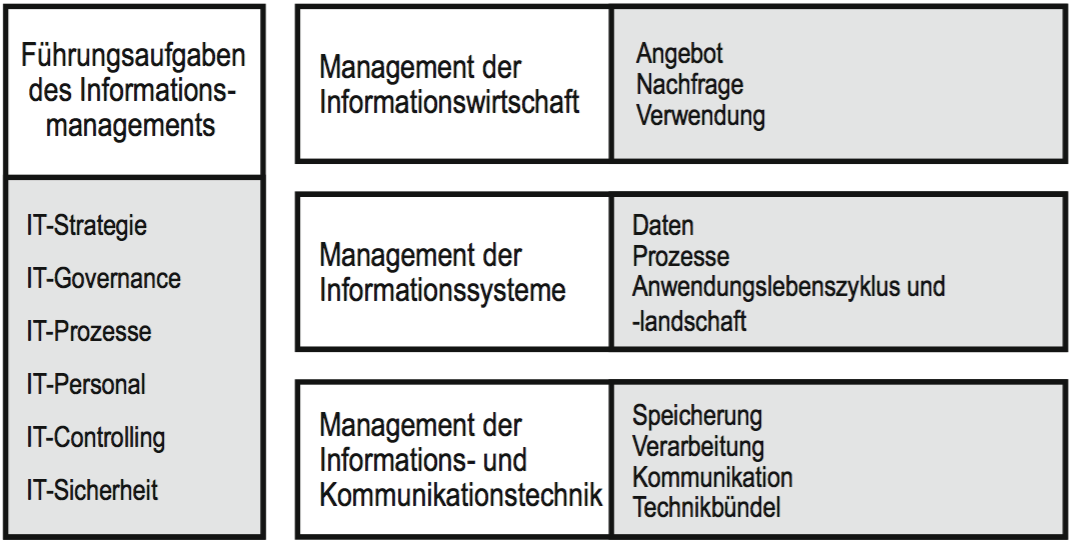
\includegraphics[width=11cm]
	{kapitel/gruppe1_1/bilder/modell_des_inm_neu}
	\caption{Modell des Informationsmanagements nach Krcmar\protect\footnotemark}
	\label{fig_modell_des_inm}
\end{figure}\footnotetext{\cite{krcmar_einfuhrung_2015}}

Das Informationsmanagement ist eine Managementaufgabe. Wie in Abbildung \ref{fig_modell_des_inm} zu sehen ist, besteht die Basis aus dem \textbf{Management der Informations- und Kommunikationstechnik}.

Auf dieser Ebene stehen die Speicherungstechnik, die Verarbeitungstechnik, die Kommunikationstechnik und die Technikbündel im Fokus.

Es wird die physische Basis für die Anwendungslandschaft auf der mittleren Ebene gelegt und damit die Bereitstellung der Informationsressourcen.

Auf der mittleren Ebene, der des Managements der Informationssysteme, liegen die Kernaufgaben im Management der Daten, der Prozesse und des Anwendungslebenszyklus. Die Ebene wird von der IKT unterstützt. Das Management der Anwendungsentwicklung erfolgt beispielsweise auf dieser Ebene.

Auf der Ebene des Managements der Informationswirtschaft besteht das Handlungsobjekt aus der Ressource Information. Es geht um den Informationseinsatz zur Deckung des Informationsbedarfs. Dieses Informationsangebot wird im Rahmen eines informationswirtschaftlichen Planungszyklus geplant, organisiert und kontrolliert.

Die Ebenen bauen also aufeinander auf. Als Ergebnis des Ordnungsrahmens können nun die einzelnen Aufgaben des Informationsmanagements identifiziert und zugeordnet werden. Die Differenzierung in drei Ebenen und einem übergreifenden Aufgabenblock zeigt, dass die Aufgaben des Informationsmanagements verteilt durchgeführt werden. Die Verteilung dieser Aufgaben gehört zur Führungsaufgabe „IT-Governance“.

Die Herstellung des informationswirtschaftlichen Gleichgewichts zwischen Informationsangebot und Informationsnachfrage bildet das Ziel des Managements der Informationswirtschaft. Das Gleichgewicht ist dynamisch, was bedeutet, dass Angebot und Nachfrage immer wieder aufeinander eingestellt werden müssen. Somit muss auch der Managementprozess der Informationswirtschaft regelmäßig ein neues Gleichgewicht suchen, sobald sich ein Parameter ändert.

Daraus ergibt sich der Lebenszyklus der Informationswirtschaft. Er besteht aus 5 Elementen aus Aktivitäten:
\begin{itemize}
	\item Management der Informationsnachfrage
	\item Management der Informationsquellen
	\item Management der Informationsressourcen
	\item Management des Informationsangebots
	\item Management der Informationsverwendung
\end{itemize}

\begin{figure}[h!]
	\centering
	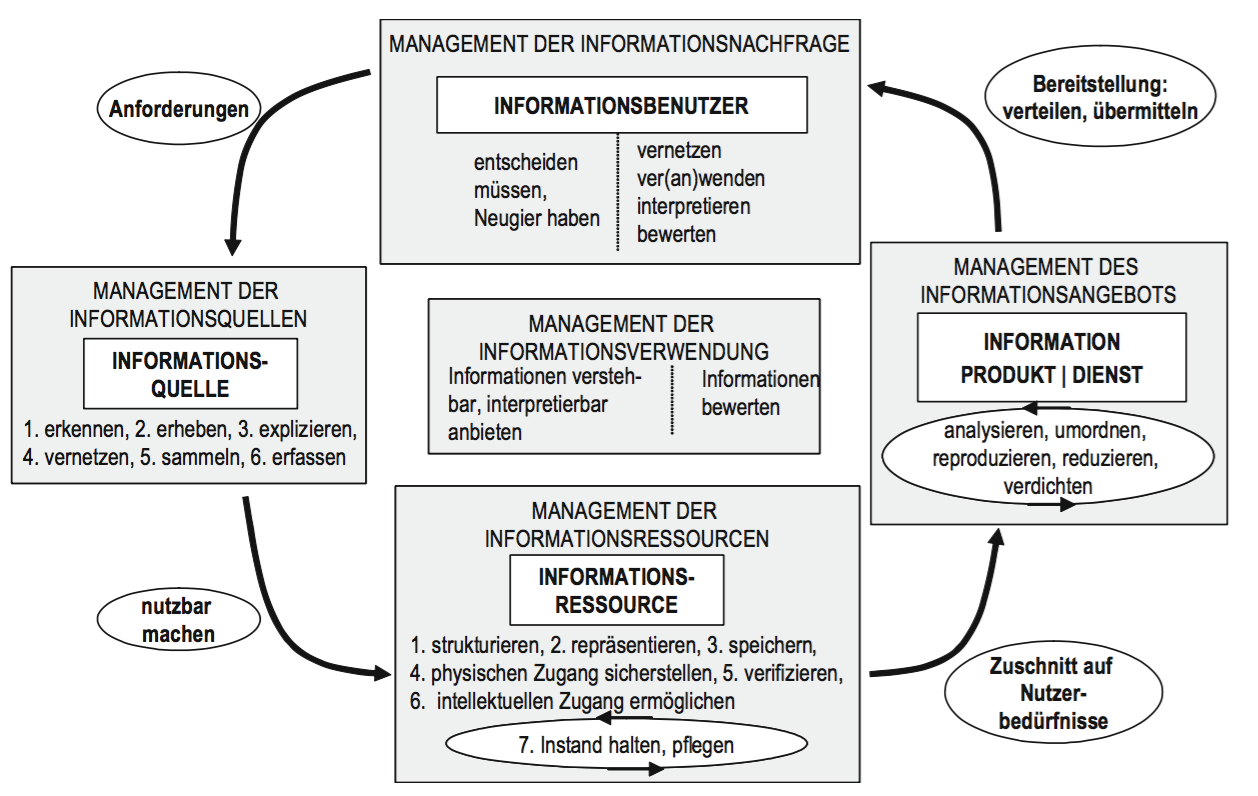
\includegraphics[width=\textwidth]
	{kapitel/gruppe1_1/bilder/lebenszyklus_der_informationswirtschaft_neu}
	\caption{Lebenszyklusmodell der Informationswirtschaft nach Krcmar\protect\footnotemark}
	\label{fig_lebenszyklus_informationswirtschaft}
\end{figure}\footnotetext{\cite{krcmar_einfuhrung_2015}}

In Abbildung \ref{fig_lebenszyklus_informationswirtschaft} lassen sich die fünf Elemente des Zyklus erkennen. Das Management der Quellen, Ressourcen, des Angebotes und der Nachfrage agieren als Teilmanagementaufgaben um das Management der Informationsressourcen.
\newpage
Stehen Informationen einem Informationsbenutzer zur Verfügung, die durch einen informationswirtschaftlichen Zyklus erschlossen wurden, kann der Informationsbedarf gedeckt werden.

Der Informationsbenutzer interpretiert die von ihm gewünschten Informationen entsprechend dem verfolgten Zweck und bringt sie zur Anwendung.
Dabei entstehen neue Informationen, da der Informationsbenutzer die angebotenen Informationen interpretiert, bewertet und mit seinen bereits vorhandenen Informationsstrukturen kombinieren kann.
Ergebnis dieser Bewertung ist, dass der Informationsbedarf gedeckt wurde oder nicht. Dementsprechend muss das Informationsangebot ausgeweitet oder verändert werden.\footcite[11-18]{krcmar_einfuhrung_2015}

\paragraph*{Software-Einführung}\mbox{}\\\\
Eine Möglichkeit für die Einführung von Software ist es, auf Standardsoftware zurück zu greifen. Andererseits können Unternehmen die Software auch selbst entwickeln, wobei Softwareentwicklungsmodelle behilflich sein können.

Der Anwendungslebenszyklus ist mit der Auswahl und Anpassung von Software noch nicht abgeschlossen., sondern erreicht die operative Nutzung erst nach erfolgreicher Einführung.

Die Einführung von Software umfasst nicht nur die Installation, sondern auch die Schulung des Personals und die Inbetriebnahme.

Zudem wird noch zwischen folgenden Konzeptionen unterschieden: 
\begin{itemize}
	\item die Stichtagsumstellung
	\item die Parallelisierung
	\item die Teilweise Einführung und
	\item die Versionsumstellung
\end{itemize}
\newpage

\paragraph*{Technochange}\mbox{}\\\\
Die Einführung von Software – im Allgemeinen von Informations- und Kommunikationstechnik-Systemen (IKT-Systemen) – kann bedeutende Veränderungen in der Arbeitsweise von Mitarbeitern auslösen. 

Diesem Prozess liegt ein hohes Leistungssteigerungspotential zugrunde, allerdings ein ebenso großes Risikopotential. 

So kann z.B. ein neu eingeführtes IKT-System von den Mitarbeitern abgelehnt werden. Diese Veränderung wird als Technochange bezeichnet, welcher 4 Phasen durchläuft.
\begin{figure}[h]
	\centering
	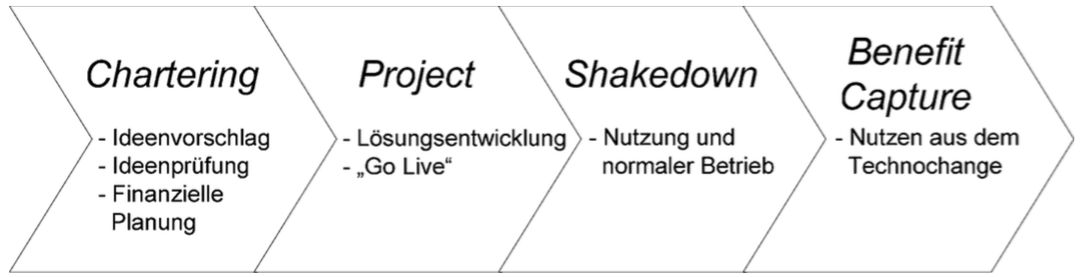
\includegraphics[width=11cm]
	{kapitel/gruppe1_1/bilder/technochange_lebenszyklus_neu}
	\caption{Technochange-Lebenszyklus nach Krcmar\protect\footnotemark}
	\label{fig_technochange_lebenszyklus}
\end{figure}\footnotetext{\cite{krcmar_einfuhrung_2015}}
In Abbildung \ref{fig_technochange_lebenszyklus} sind diese Phasen zu sehen. Der Lebenszyklus ist eigentlich eher ein Lebenslauf, in dem die einzelnen Phasen – Chartering, Project, Shakedown und Benefit Capture – aufeinander aufbauen.

\paragraph*{Softwareentwicklungsmodelle}\mbox{}\\\\
Gut geplante Einzelschritte des Projekts und die Einkalkulation ggf. entstehende Probleme und deren Lösungsfindung entscheiden wesentlich über den Erfolg einer Anwendungsentwicklung.
Aufgrund der Dynamik innerhalb des Entwicklungsprozesses, muss die Projektplanung laufend aktualisiert werden.

Meilensteine, Ergebnisse, Ziele und Kriterien werden vor Beginn der Projektphase festgelegt. Verschiedene Optionen zur Projektdurchführung sind anhand der Kriterien zu bewerten und gegenüber zu stellen, und zwar sowohl vor Projektbeginn, als auch im Laufe des Projekts.

Im weiteren Verlauf durchläuft das Projekt einen Software-Zyklus mit mehreren Stadien.  Iterative Modelle haben sich in der Praxis durchgesetzt, mit fest definierten Phasen, die sequenziell durchlaufen werden.

Das Wasserfallmodell wurde durch die Integration qualitätssichernder Maßnahmen 1992 zum V-Modell weiterentwickelt und 1997 überarbeitet. Die Strukturierung anhand des V-Modells erfolgt anhand drei Ebenen:

Vorgehensweise (Was ist zu tun?)

Methode (Wie ist es zu tun?)

Werkzeuganforderungen(Womit ist etwas zu tun?)

Um die meist sehr komplexe Aufgabe erfolgreich umzusetzen, muss eine geeignete Projektorganisation aufgebaut werden.

Da die Einführung von Software eine besondere Herausforderung für Unternehmen mit sich bringt, sind Vorgehensmodelle von außerordentlicher Bedeutung. 
Diese haben das Ziel, den Ablauf einer Softwareentwicklung zu beschreiben und den Prozess zur Softwareentwicklung in handhabbare Teilaufgaben zu strukturieren. 
Dabei kann zwischen stark und weniger stark formalisierten sowie sequenziellen oder initiativen Vorgehensmodellen stark unterschieden werden. 
Die bedeutendsten Vorgehensmodelle sind das V-Modell, das Spiralmodell sowie der Rational Unified Process (RUP).

Ferner ist es notwendig die Einführung von Software wirtschaftlich zu rechtfertigen. Anhand von Verfahren zur Kostenschätzung können die Kosten für Entwicklung, Erwerb und Nutzung von Informationssystemen geschätzt werden und dadurch deren Wirtschaftlichkeit gerechtfertigt werden.\footcite[80 ff.]{krcmar_einfuhrung_2015}

Auch an Hochschulen ist es von großer Wichtigkeit das Gleichgewicht von Informationsangebot und -nachfrage in Balance halten zu können. 
Das hier ebenfalls dynamische Gleichgewicht ist an den Informationsbedarf der Hochschulangehörigen angelehnt. 
Dieser Personenkreis umfasst nicht nur die Studenten, sondern auch die Hochschulangestellten. 
Es ist Aufgabe des Hochschulpersonals die Informationsnachfrage der Studierenden und Studienbewerber mit einem Informationsangebot zu decken, welches bezüglich der Qualität der Informationen eine Bedarfsdeckung verspricht. 
Die Entscheidung, ob Standardsoftware verwendet werden soll, oder ob sie hochschulintern entwickelt werden soll, ist unter den Hochschulen individuell getroffen. 
Es gilt gewisse Faktoren zu beachten, die in den Entscheidungsprozess Einfluss nehmen, wie beispielsweise der zeitliche Aufwand der Entwicklung, Testphasen oder die Kosten. 
Die bereits genannten Softwareentwicklungsmodelle tragen zur Entscheidungshilfe bei.
Die Einführung einer Software kann einen Technochange beinhalten und birgt dadurch große Risiken. 
Der Mensch ist nur ungern von seinen Gewohnheiten abzubringen, wodurch auch die Umstellung hochschulinterner Systeme Frustration und Unmut auslösen kann, was den Arbeitsaufwand der Studentenbetreuung erhöht.
\newpage
